\documentclass[10pt,xcolor={dvipsnames,table},aspectratio=169]{beamer}

%\usetheme{Boadilla}
%\usecolortheme{wolverine}
\usecolortheme{dolphin}
%\setbeamercovered{transparent}
%\setbeamercolor{block body}{bg=yellow}

\addtobeamertemplate{navigation symbols}{}{%
	\usebeamerfont{footline}%
	\usebeamercolor[fg]{footline}%
	\hspace{1em}%
	\insertframenumber/\inserttotalframenumber
}

\usepackage{fontspec}
\defaultfontfeatures{Renderer=Basic,Ligatures={TeX}}
%    \setmainfont{CMU Serif}
%    \setsansfont{CMU Sans Serif}
\setmainfont{DejaVu Serif}
\setsansfont{CMU Sans Serif}
%    \setmonofont{CMU Typewriter Text}
\usepackage{unicode-math}
%    \setmathfont{Latin Modern Math}
%    \setmathfont{Libertinus Math}
%    \setmathfont{TeX Gyre DejaVu Math}
\setmathfont{STIX Two Math}
\usepackage[english,russian]{babel}
\usepackage{graphicx}
\usepackage{wrapfig}
\usepackage{animate}
\usepackage{ragged2e}
\usepackage{color}
\usepackage{pgfplots}
\usepackage{subcaption}
\usepackage[font=small,labelfont=bf]{caption}
\usepackage{svg}
\usepackage{listings}

\usepackage{tikz}
%\usetikzlibrary{
	%	mindmap,
	%	arrows, % стрелки
	%	shapes.misc, % фигуры
	%	chains, % цепочки
	%	positioning, % позиционирование элементов
	%	scopes, % создание дополнительных веток
	%	shadows % тени
	%}

\graphicspath{{pic/}{figs/}}

\author[Губкин]{А.С.~Губкин}

\title[Расчёт коэффициента теплоотдачи прямого канала прямоугольного сечения]{Расчёт коэффициента теплоотдачи прямого канала прямоугольного сечения}

\date[Тюмень 2024]{Июль, 2024 г.}

\begin{document}
    \frame{\titlepage}

    %SLIDE #
    \begin{frame}{}

        %\transdissolve[duration=0.1]
        \justifying
        \normalsize

        \frametitle{Задача}

        Определить коэффициент теплоотдачи $ \tilde{\alpha} $ прямого канала длиной $ l~=~400$~мм прямоугольного сечения ширины $ w~=~15 $~мм и высоты $ h~=~8 $~мм с толщиной стенки $ \delta_{wall}~=~1 $~мм при протекании через него диоксида углерода. Скорость и температура газа на входе в канал соответственно $ u_{inlet}~=~20 $~м/с, $ T_{inlet}~=~423.15 $~К. Давление на выходе из канала $ p_{outlet}~=~4 $~МПа. Канал обменевается энергией с внешней средой при температуре $ T_{ext}~=~723.15 $~К с коэффициентом теплоотдачи $ \alpha_{ext}~=~1000 $~Вт/м$^2$К.

    \end{frame}

    %SLIDE #
    \begin{frame}

        %\transdissolve[duration=0.1]
        \justifying
        \normalsize

        \frametitle{Фазовая диаграмма $CO_{2}$}

        \begin{minipage}[b]{0.49\linewidth}
            Из фазовой диаграммы диоксида углерода видно, что при данном режиме фазовые переходы отсутствуют. Течение будет происходить в газовой фазе. \\

            Параметры критической точки: $ p_{c}~=~7.3773 $~МПа, $ T_{c}~=~304.128 $~К, $ V_{c}~=~0.09412 $~м$^{3}$/кмоль.
        \end{minipage}
        \hfill
        \begin{minipage}{0.49\linewidth}
            \begin{figure}
                \centering
                \includesvg[scale=0.4]{Carbon_dioxide_pressure-temperature_phase_diagram}
            \end{figure}
        \end{minipage}

    \end{frame}

    %SLIDE #
    \begin{frame}{}

        %\transdissolve[duration=0.1]
        \justifying
        \normalsize

        \frametitle{Уравнение состояния}

        Будем использовать уравнение Пенга - Робинсона (англ.~Peng–Robinson, 1976)

        \[
            \rho = \frac{p}{Z \left( p, T \right) \bar{R} T}
        \]

        \[
            Z^{3} - \left( 1 - B \right) Z^{2} + \left( A - 2B - 3B^{2} \right) Z - \left( AB - B^{2} - B^{3} \right) = 0
        \]

        \[
            A = \frac{\alpha a p}{R^{2} T^{2}}, \: B = \frac{b p}{R T}
        \]

        \[
            a = \Omega_{a} \frac{R^{2} T^{2}_{c}}{p_{c}}, \:
            \Omega_{a} = \frac{8 + 40 \eta_{c}}{49 - 37 \eta_{c}}
            b = \Omega_{b} \frac{R T_{c}}{p_{c}}, \:
            \Omega_{b} = \frac{\eta_{c}}{3 + \eta_{c}}
        \]

        \[
            \eta_{c} = \left( 1 + \left( 4 - \sqrt{8} \right)^{\frac{1}{3}} + \left( 4 + \sqrt{8} \right)^{\frac{1}{3}} \right)^{-1}
        \]

        \[
            \alpha = \left( 1 + \kappa \left( 1 - \sqrt{T_{r}} \right) \right)^{2}, \: T_{r} = \frac{T}{T_{c}}
        \]

        \[
            \kappa = 0.37464 + 1.54226 \omega - 0.26992 \omega^{2}
        \]

    \end{frame}

    %SLIDE #
    \begin{frame}{}

        %\transdissolve[duration=0.1]
        \justifying
        \normalsize

        \frametitle{Оценка числа Рейнольдса и величины подслоя}

        \[
            Re = \frac{u_{0} d}{\nu} = \frac{20 \sqrt{0.008^{2} + 0.015^{2}}}{1.5 \cdot 10^{-5}} \approx 22666
        \]

        \[
            \delta = \delta_{T} \approx \frac{0.37 x}{Re^{\frac{1}{5}}_{x}} = \left. \frac{0.37 x}{\left( \frac{u_{0} x}{\nu} \right)^{\frac{1}{5}}} \right|_{x = l} = \frac{0.37 x}{\left( \frac{20 \cdot 0.4}{1.5 \cdot 10^{-5}} \right)^{\frac{1}{5}}} = \approx 0.011
        \]

    \end{frame}

    %SLIDE #
    \begin{frame}{}

        %\transdissolve[duration=0.1]
        \justifying
        \normalsize

        \frametitle{Математическая модель}

        \[
            \left.
            \begin{aligned}
                &\frac{\partial \rho}{\partial t}
                + \symbf{\nabla} \cdot \symbf{\rho u} = 0 \\
                &\frac{\partial \rho \symbf{u}}{\partial t}
                + \symbf{\nabla} \cdot \rho \symbf{u} \otimes \symbf{u}
                =
                - \symbf{\nabla} p
                + \symbf{\nabla} \cdot \symbf{\tau}\\
                &\frac{\partial \rho E}{\partial t}
                + \symbf{\nabla} \cdot \rho \symbf{u} E
                + \symbf{\nabla} \cdot \symbf{u} p
                =
                - \symbf{\nabla} \cdot \symbf{q}
                + \symbf{\nabla} \cdot \symbf{\tau \cdot \symbf{u}}\\
                &\symbf{\tau} = \mu_{eff} \left[ \symbf{\nabla} \symbf{u} + \left( \symbf{\nabla} \symbf{u} \right) ^{T}  - \frac{2}{3} \left(  \symbf{\nabla} \cdot \symbf{u} \right) \symbf{I} \right], \: \mu_{eff} = \mu + \mu_{t}
            \end{aligned} \right\rbrace \quad \symbf{x} \in \Omega_{flow}
        \]

        \[
            \frac{\partial \rho_{s} c_{s} T}{\partial t} + \symbf{\nabla} \cdot \lambda_{s} \symbf{\nabla} T = 0 \quad \symbf{x} \in \Omega_{Solid}
        \]

    \end{frame}

    %SLIDE #
    \begin{frame}[fragile]

        %\transdissolve[duration=0.1]
        \justifying
        \normalsize

        \frametitle{}

        \[
             \mu = \frac{A_{s} \sqrt{T}}{1 + \frac{T_{s}}{T}}
        \]

        \[
            \lambda = \mu c_{v} \left( 1.32 + 1.77 \frac{R}{c_{v}} \right)
        \]

        \[
            A_{s} = 1.67212 \cdot 10^{-6}, \: T_{s} = 170.6
        \]

        \[
            c_{p} = ((((a_{4} T + a_{3}) T + a_{2}) T + a_{1}) T + a_{0}) + c_{p, eos}
        \]
        {\centering\scriptsize
        \begin{lstlisting}
thermodynamics
{
    Tlow            0;
    Thigh           5000;
    Tcommon         1000;
    highCpCoeffs    (3.85746 0.00441437 -2.21481e-06 5.2349e-10 -4.72084e-14 -48759.2 2.27164);
    lowCpCoeffs     (2.35677 0.0089846 -7.12356e-06 2.45919e-09 -1.437e-13 -48372.0 9.90105);
}
        \end{lstlisting}
        }

    \end{frame}

    %SLIDE #
    \begin{frame}{}

        %\transdissolve[duration=0.1]
        \justifying
        \normalsize

        \frametitle{Модель турбулентности}

        \[
            \begin{aligned}
                &\frac{\partial \rho k}{\partial t}
                + \symbf{\nabla} \cdot \rho k \symbf{u}
                =
                \symbf{\nabla} \cdot \left[ \left(\mu + \frac{\mu_{t}}{\sigma_k} \right) \symbf{\nabla} k \right]
                + 2 \mu_{t} \symbf{S} \colon \symbf{S} \ - \rho \varepsilon  \\
                &\frac{\partial \rho \varepsilon}{\partial t}
                + \symbf{\nabla} \cdot \rho \varepsilon \symbf{u}
                =
                \symbf{\nabla} \cdot \left[\left(\mu + \frac{\mu_{t}}{\sigma_{\varepsilon}} \right) \symbf{\nabla} \varepsilon \right]
                + C_{1 \varepsilon} \frac{\varepsilon}{k} 2 \mu_{t} \symbf{S} \colon \symbf{S} - C_{2 \varepsilon} \rho \frac{\varepsilon^2}{k}
            \end{aligned}
        \]

        \[
            \mu_{t} = \rho C_{\mu} \frac{k^{2}}{\varepsilon}
        \]

        \[
            C_{1 \varepsilon} = 1.44, \; C_{2 \varepsilon} = 1.92, \; C_{\mu} = 0.09, \; \sigma_{k} = 1.0, \; \sigma_{\varepsilon} = 1.3
        \]

    \end{frame}

    %SLIDE #
    \begin{frame}{}

        %\transdissolve[duration=0.1]
        \justifying
        \normalsize

        \frametitle{Сетка}
        
        Общее количество контрольных объемов 416400. Количество контрольных объемов в области течения и стенке соответственно 228800 и 187600. Гексаэдров: 308800. Призм: 107600.

        \begin{minipage}{0.45\linewidth}
            \begin{figure}
                \centering
                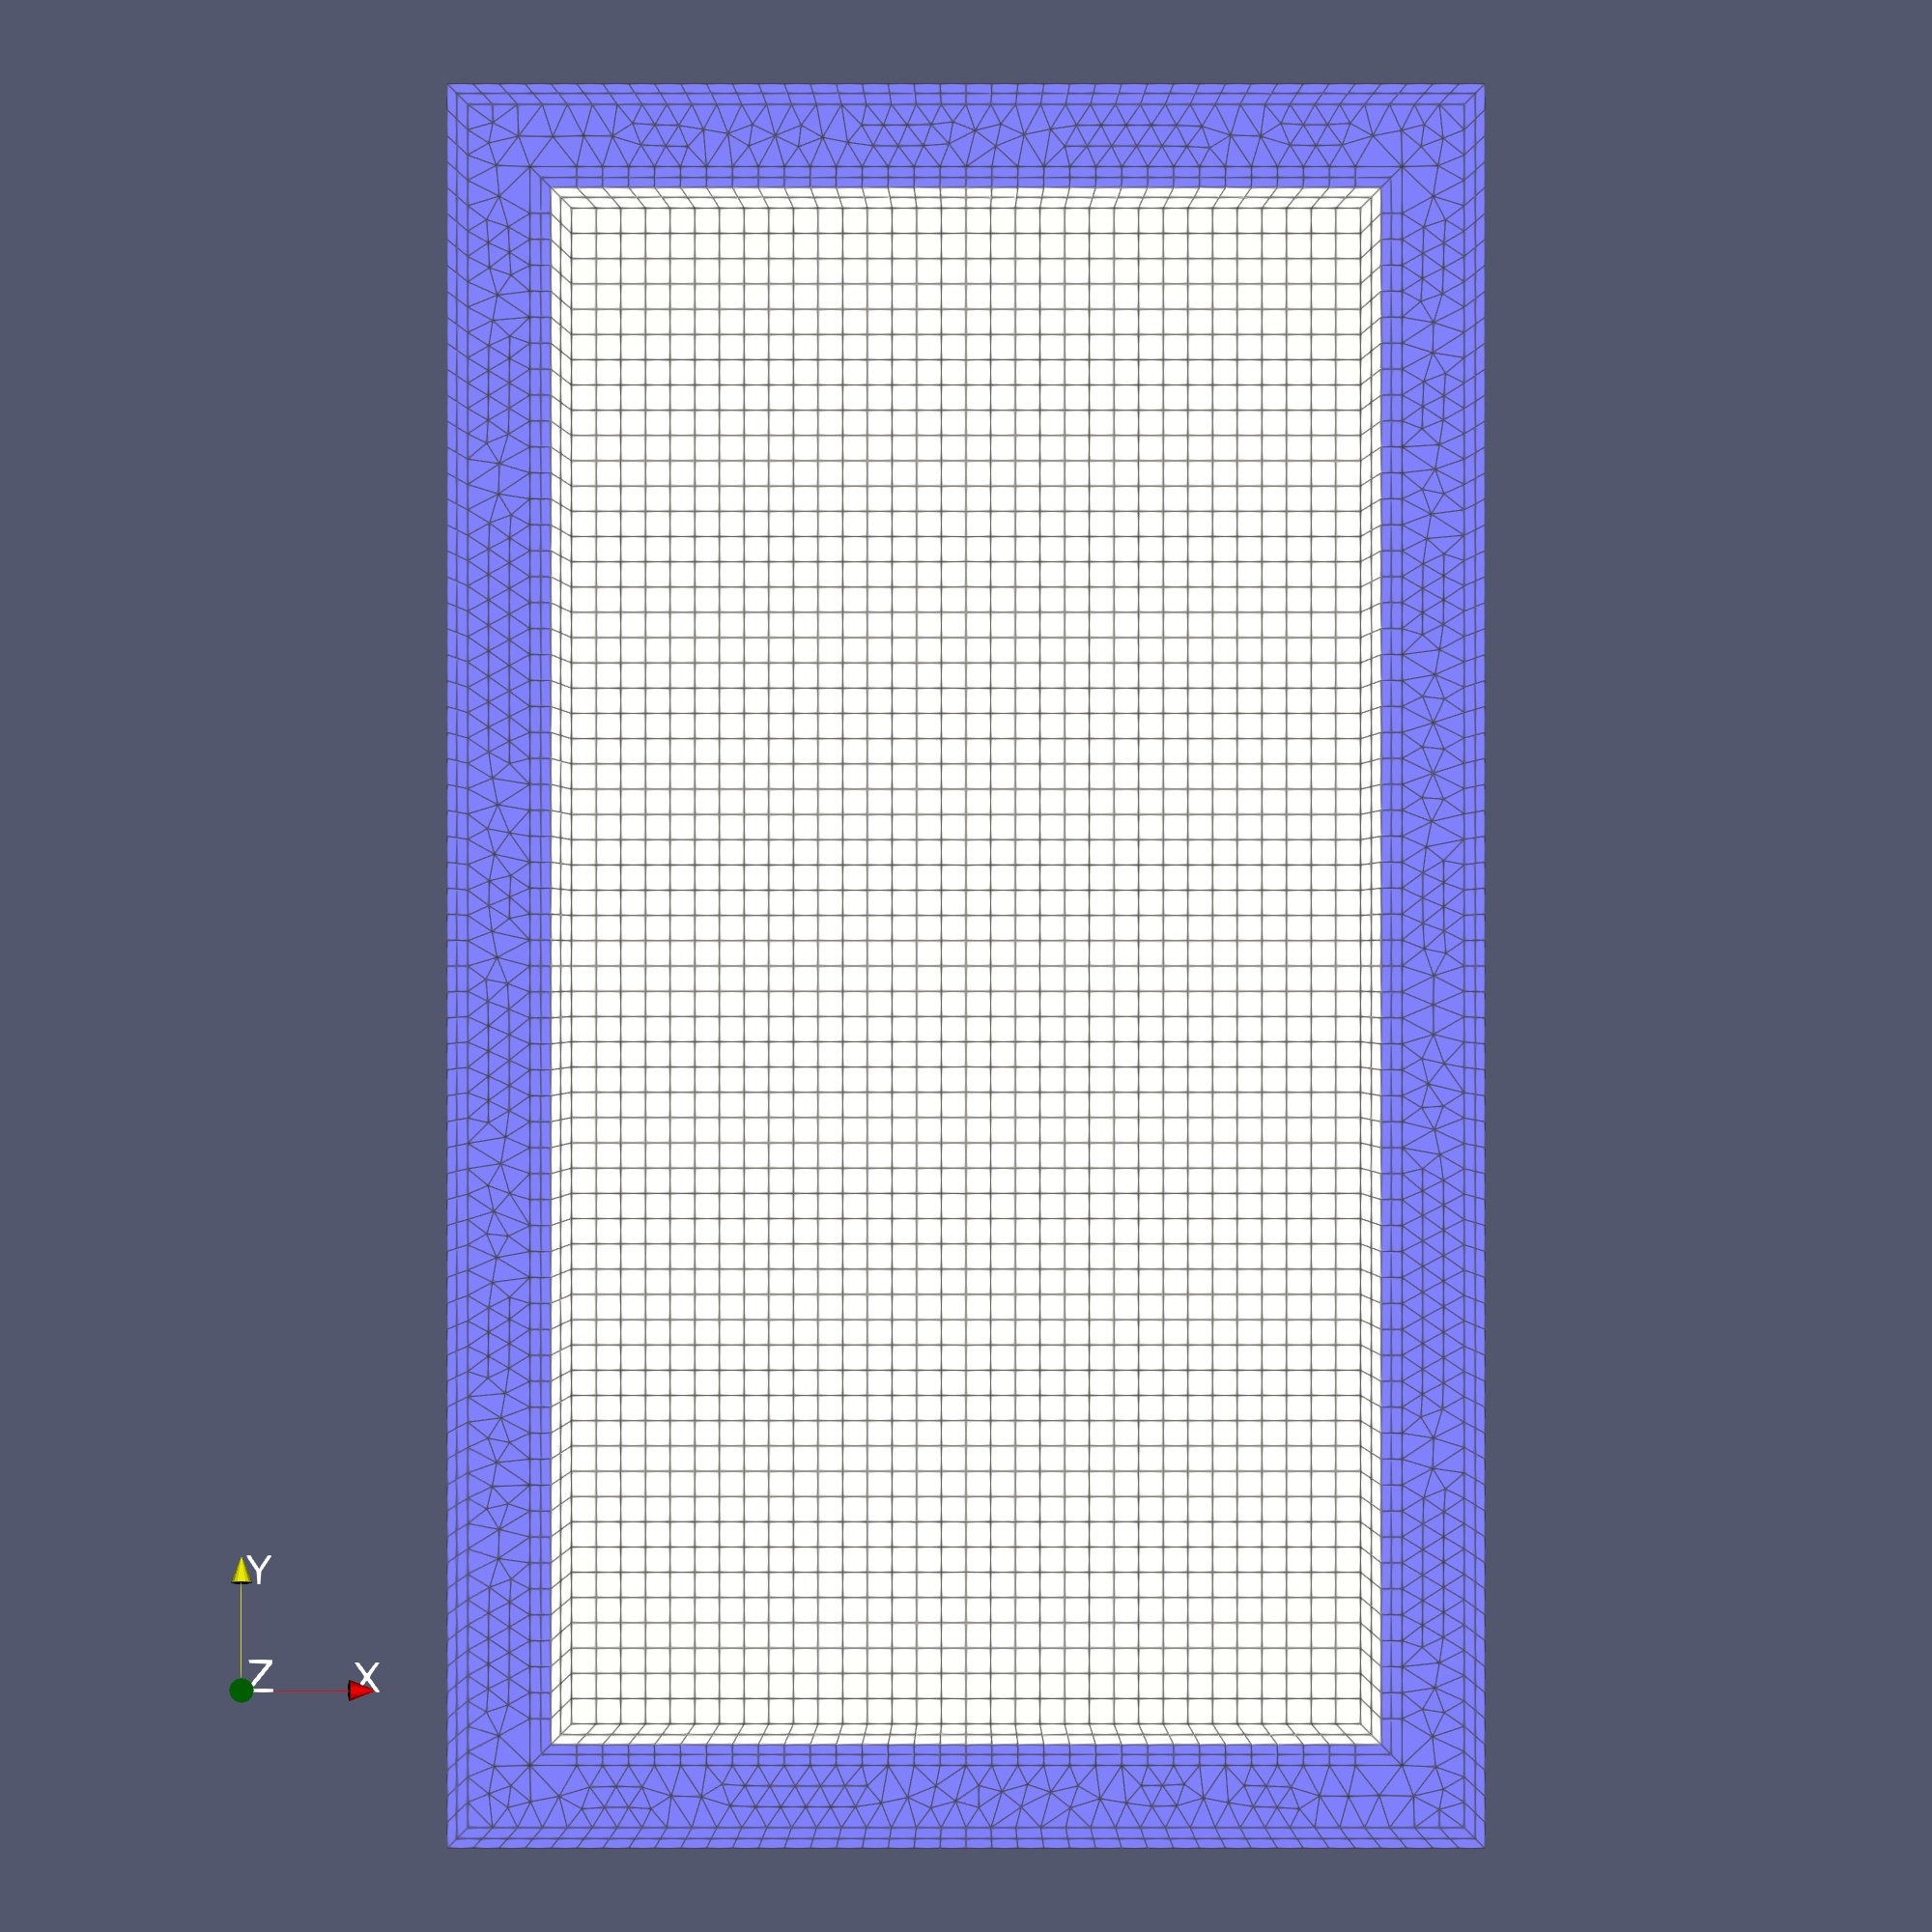
\includegraphics[scale=0.08]{mesh1}
            \end{figure}
        \end{minipage}
        \hfill
        \begin{minipage}{0.45\linewidth}
            \begin{figure}
                \centering
                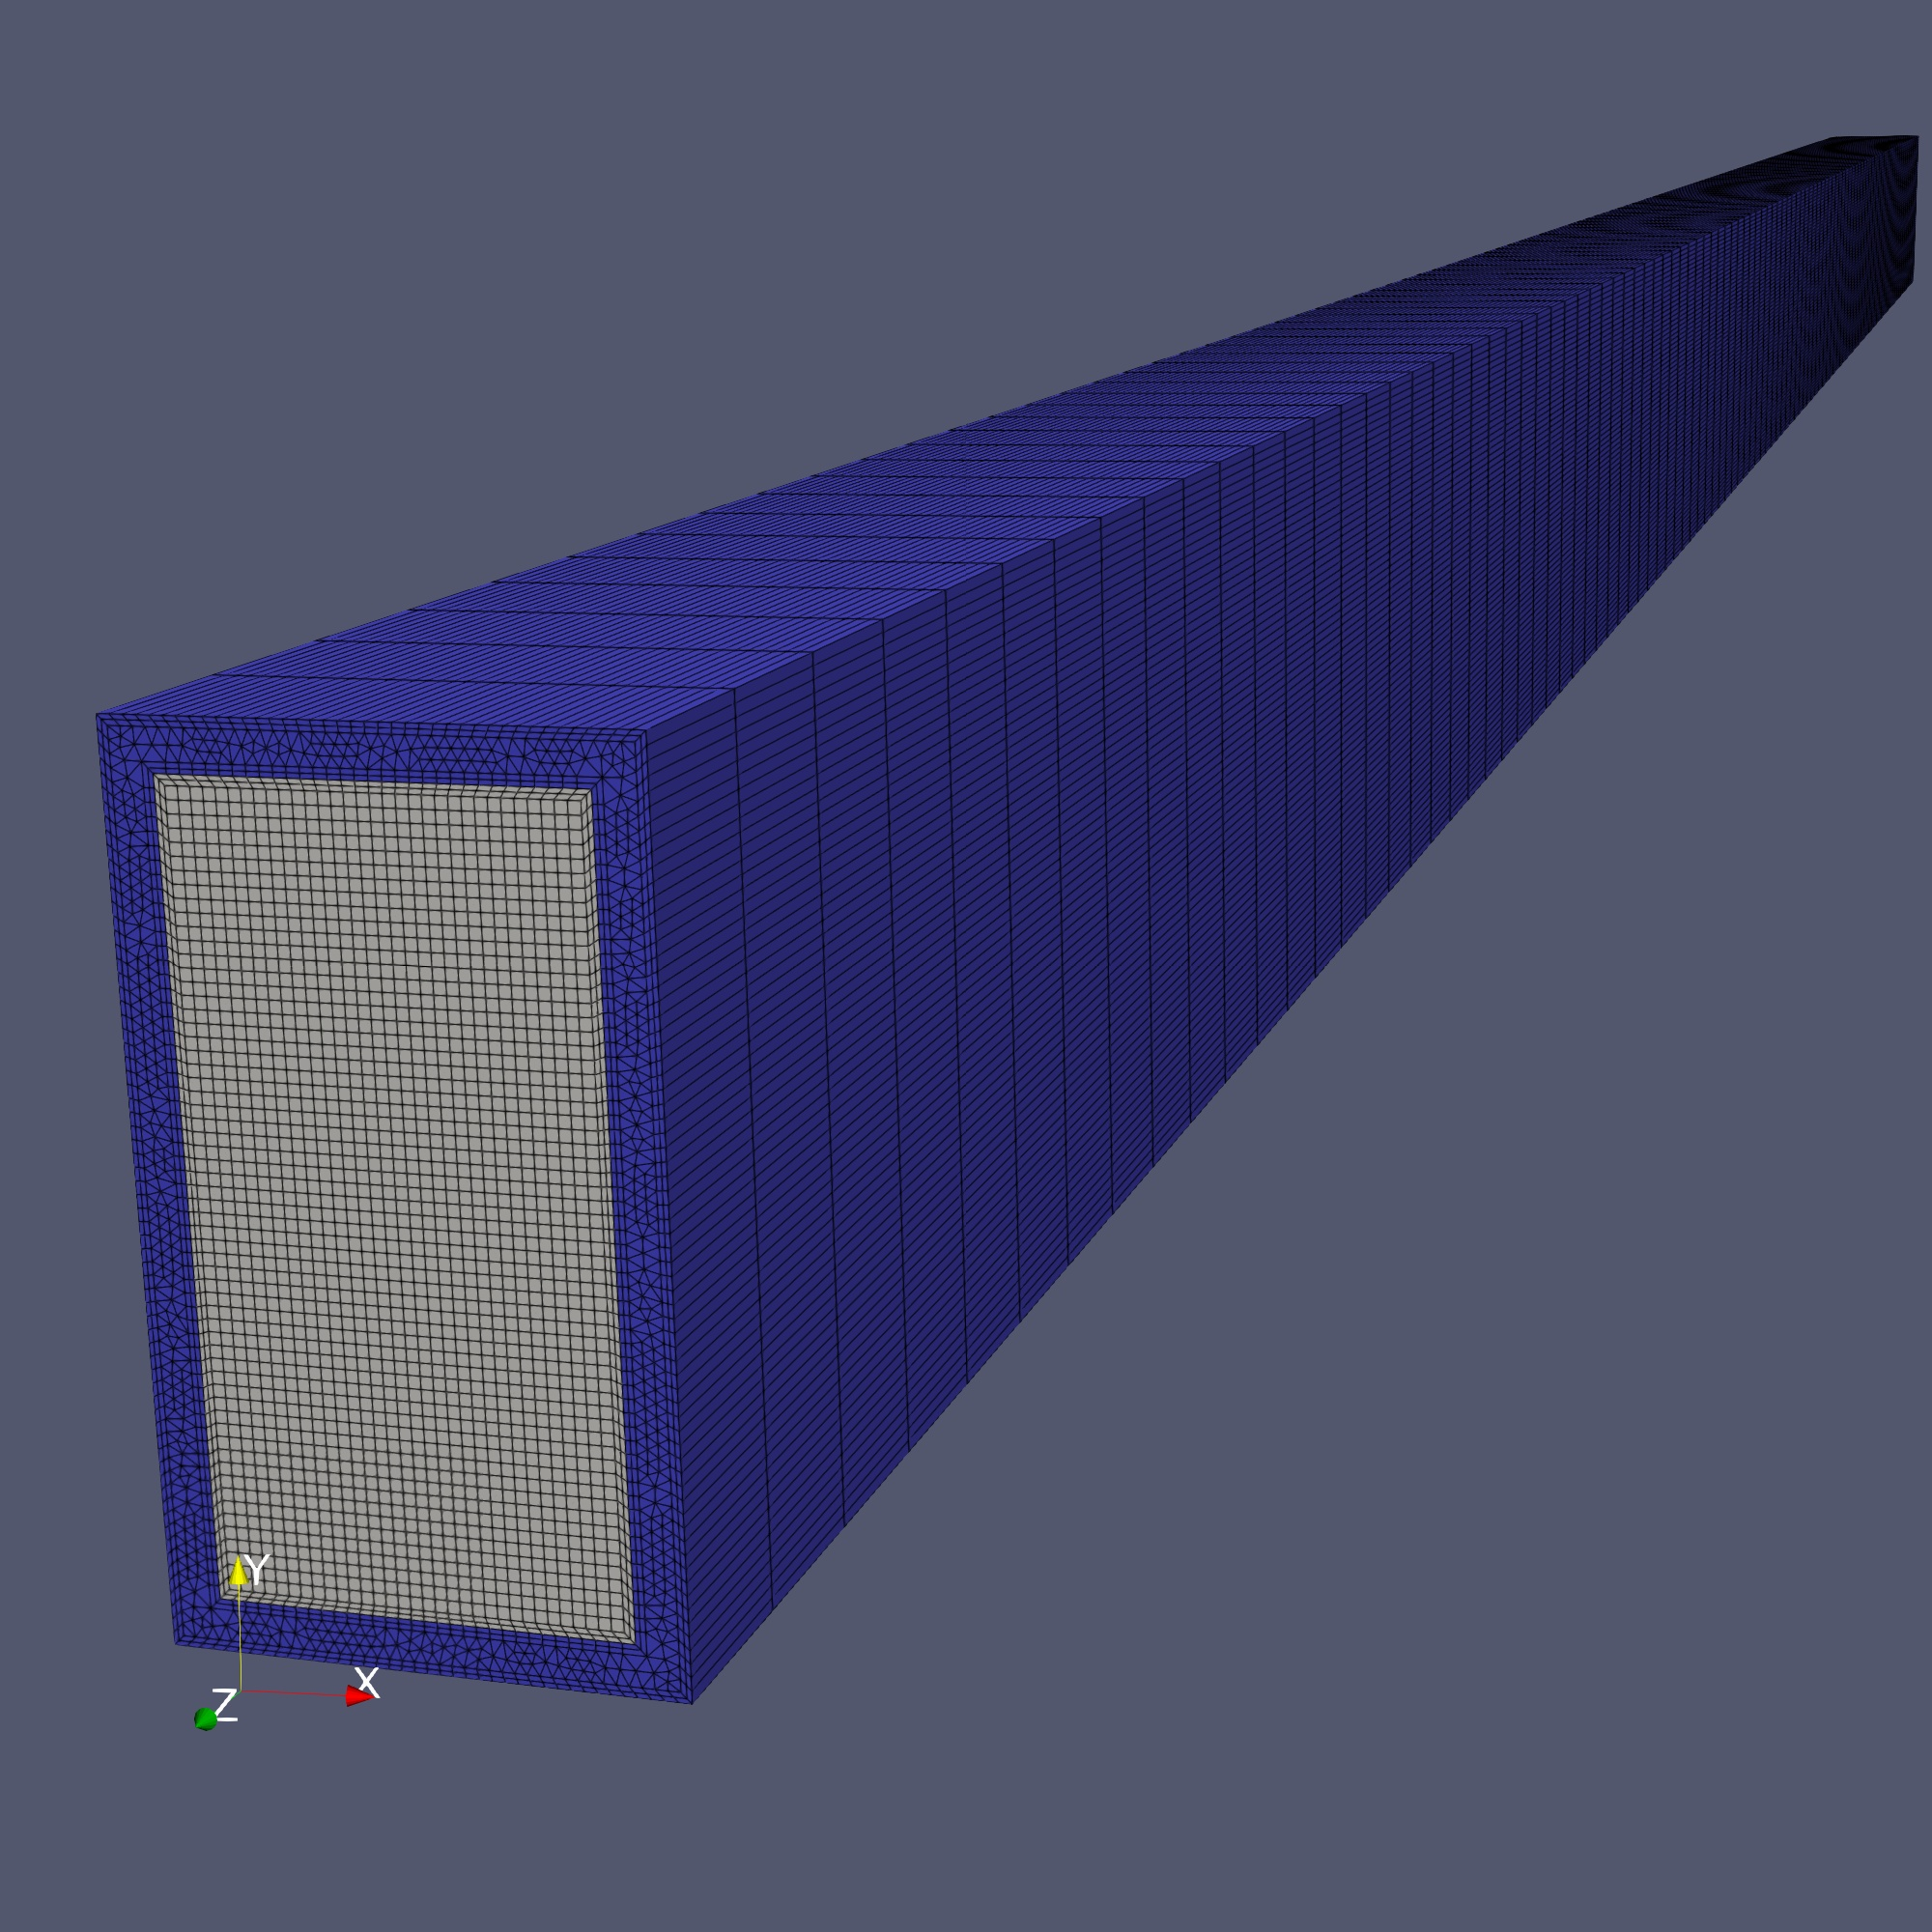
\includegraphics[scale=0.08]{mesh2}
            \end{figure}
        \end{minipage}

    \end{frame}
    
%    %SLIDE #
%    \begin{frame}{}
%
%        %\transdissolve[duration=0.1]
%        \justifying
%        \normalsize
%
%        \frametitle{Граничные условия}
%
%        \[
%            \begin{aligned}
%                &\begin{aligned}
%                    &\symbf{u} = 0 \\
%                    \symbf{\nabla} &p = 0
%                \end{aligned} \quad \symbf{x} \in \partial \Omega_{wall} \\
%                &\begin{aligned}
%                    \symbf{\nabla} &\symbf{u} = 0 \\
%                    &p = p_{1}
%                \end{aligned} \quad \symbf{x} \in \partial \Omega_{inlet} \\
%                &\begin{aligned}
%                    \symbf{\nabla} &\symbf{u} = 0 \\
%                    &p = p_{2}
%                \end{aligned} \quad \symbf{x} \in \partial \Omega_{outlet}
%            \end{aligned}
%        \]
%
%    \end{frame}

    %SLIDE #
    \begin{frame}{}

        %\transdissolve[duration=0.1]
        \justifying
        \normalsize

        \frametitle{Расчет коэффициента теплоотдачи}

        \[
            \alpha = \frac{\rho c_{p}}{\delta_{wall}} \left( \frac{\nu}{\textsf{Pr}} + \frac{\nu_{t}}{\textsf{Pr}_{t}} \right)
        \]

        \[
            \tilde{\alpha} = \frac{1}{S_{wall}} \int\limits_{S_{wall}} \alpha \approx 141.27 \; \frac{\mbox{Вт}}{\mbox{м}^2 \: \mbox{К}}
        \]

    \end{frame}

\end{document}